%%%%%%%%%%%%%%%%%%%%%%%%%%%%%%%%%%%%%%%%%%%%%%%%%%%%%%%%%%%%%
%% Der Teufel steckt im Detail -- F.N.                     %%
%%%%%%%%%%%%%%%%%%%%%%%%%%%%%%%%%%%%%%%%%%%%%%%%%%%%%%%%%%%%%
%%%%%%%%%%%%%%%%%%%%%%%%%%%%%%%%%%%%%%%%%%%%%%%%%%%%%%%%%%%%%
%%															%%                         %%				
%%			école —————————————			%%                         %%
%%			normale ———————————			%%                         %%
%%			supérieure ————————			%%                         %%
%%			paris—saclay ——————			%%                         %%
%%															%%                         %%
%%%%%%%%%%%%%%%%%%%%%%%%%%%%%%%%%%%%%%%%%%%%%%%%%%%%%%%%%%%%%

\documentclass[11pt,a4paper]{article}
\usepackage[utf8]{inputenc} 				%% Single Byte Per Letter. Use Unicode if you are not using listings
\usepackage[french]{babel}
\usepackage[T1]{fontenc}

\usepackage[a4paper]{geometry}
\usepackage{listings}									%% Best way to include code

%\usepackage{colortbl}									%% Colored tables
\usepackage{xcolor}										%% Extended color
\usepackage{framed}										%% For frames

\newif\iffancy
\fancyfalse

\iffancy
\usepackage{fancyhdr}									%% Fancy Header
\pagestyle{fancy}
\setlength{\headheight}{15pt}
%% ATTENTION
%%	The following \sectitle refers to the title
%%  of the subsection setted from \newsubsection
%% 	It allows the text of this subsection to be 
%%	written in the header.
\lhead{Left}
\chead{Center}
\rfoot{\textit{\thesubsection \phantom{W} \sectitle}}
%\else
%\pagestyle{headings}
\fi
\usepackage{bbold}										%%
\usepackage{lmodern}									%% cmbright, charter, mathptmx
%\usepackage{slashbox}									%% Double entry tables
%\usepackage{array,multirow,makecell}	%% Extended options for tables
\usepackage[a4paper]{geometry}
\usepackage{stmaryrd}
\usepackage{amsthm,amsmath,amsfonts,amssymb}
%\usepackage{xspace}										%% In case of \newcommand{}{}
\usepackage[hidelinks]{hyperref}
\definecolor{violet}{rgb}{0.5,0,0.5} 

\newtheorem{ex}{Exercice}
%% Details
\AddThinSpaceBeforeFootnotes 
\FrenchFootnotes

%% Colors
\definecolor{lightgreen}{rgb}{0.5,1.0,0.5} 
\definecolor{lightred}{rgb}{1.0,0.5,0.5} 
\definecolor{fond}{gray}{0.85} 
\newenvironment{cadrecode}
{
%pour tracer des barres verticales devant un $ 
\def\FrameCommand{{\color[HTML]{888888}\vrule width 3pt}\colorbox{fond}}% 
\MakeFramed {\advance\hsize-\width \FrameRestore}}% 
{\endMakeFramed} 

\newcommand{\sectitle}{}
\newcommand{\newsubsection}[1]
{\subsection{#1}\renewcommand{\sectitle}{#1}}

\newcommand{\remark}[1]{\begin{cadrecode}{#1} \end{cadrecode}}





\lstset{language=c++,
basicstyle=\ttfamily,
breaklines=true,
keepspaces=true,
tabsize=2,
morekeywords={set, subject, param, var, in, to, union},
keywordstyle=\color{blue},
commentstyle=\color[gray]{0.25},
stringstyle=\color{purple},
extendedchars=true}


\newcommand{\f}[1]{\lstinline{#1}}


\title{Groupes de discussion par inondation fiable : NetGDIF}
\author{Adam \bsc{Phillips}, Vincent \bsc{Bonczak}}

\begin{document}
  \maketitle
	
	\begin{abstract}
	Ce document présente notre implémentation du projet de Réseaux de l'année 2020-2021 à l'École Normale Supérieure Paris-Saclay. Dans une première partie
	nous revenons sur l'état général du projet et ce qui a pu être effectivement réalisé, par rapport à notre ambition de départ. La seconde partie traite 
	des détails d'implémentation et des difficultés rencontrées lors de la phase de programmation du protocole. On trouvera enfin en conclusion de ce rapport
	des remarques à propos des tests effectuées, nos réserves quant au comportement actuel du programme, ainsi que quelques perspectives envisageables.
	\end{abstract}
	
	
\section{Introduction}

L'implémentation d'un système de discussion publique et distribué comporte plusieurs parties dont la plus importante reste la mise en œuvre d'un algorithme \emph{distribué}. Pour ce projet, le sujet fournissait cet algorithme, restait donc l'implémentation.

Cette dernière a été réalisée en C++\footnote{Standard C++14.} à l'aide  des fonctions de la bibliothèque standard, ainsi que de la bibliothèque d'affichage en mode texte \texttt{ncurses}.

\subsection{État du projet}


Le sujet minimal a été suivi, avec quelques extensions détaillées dans la suite. Nous n'avons cependant pas couvert IPv4 (en fait le pair exige une adresse IPv6). Cependant si un pair géré par
une autre implémentation que la nôtre communique avec nous en IPv4, nous sommes en mesure de le recevoir -- à supposer qu'il puisse envoyer dans un multicast 
idoine pour ses Hello courts -- et de communiquer son adresse aux voisins\footnote{Sous forme \emph{IPv4-Mapped}.} 

En outre, nous avons développé les extensions suivantes (en plus de la sécurité de l'implémentation) :
\begin{description}
\item[Agrégation] Les TLV sont placés dans une liste d'attente (\f{toSend}) indexée par les adresses de destination. Pour chaque destinataire, la fonction \f{sendPendingTLVs}
envoie le plus de TLV possible dans un paquet UDP. Si il n'y a pas assez de TLV, elle remplit au minimum le paquet avec un PadN de 255 octets.
\item[Découverte multicast]Les Hello courts sont envoyés en multicast sur le port 1212.

\item[Fragmentation] Il est possible d'envoyer des messages de plus de 254 caractères grâce à un mécanisme de fragmentation sommaire qui envoie autant de 
TLV Data que nécessaire\footnote{La remise dans l'ordre n'est cependant pas au point.}.
\end{description}

Nous nous sommes intéressés également au transfert de fichier, mais sans aller au bout : voici néanmoins notre proposition pour effectuer ce type de transfert:

\begin{lstlisting}
#define TLV_FILE			0xf1      //Identifiant du TLV
\end{lstlisting}

Tout d'abord, réserver un identifiant. Le TLV File sert à échanger des requêtes pour déterminer les personnes intéressées par le fichier (il n'est pas question
d'écrire sans préavis sur la machine du pair). Ce TLV a le format suivant :

\begin{verbatim}
0                   1                   2                   3
0 1 2 3 4 5 6 7 8 9 0 1 2 3 4 5 6 7 8 9 0 1 2 3 4 5 6 7 8 9 0 1
+-+-+-+-+-+-+-+-+-+-+-+-+-+-+-+-+-+-+-+-+-+-+-+-+-+-+-+-+-+-+-+-+
| Type = 0xf1   |     Length    |     Step      |     RESV      |
+-+-+-+-+-+-+-+-+-+-+-+-+-+-+-+-+-+-+-+-+-+-+-+-+-+-+-+-+-+-+-+-+
|          Sequence number      |           Data    ...	         
+ +-+-+-+-+-+-+-+-+-+-+-+-+-+-+-+-+-+-+-+-+-+-+-+-+-+-+
\end{verbatim}

Le champ \texttt{Step} identifie à quelle étape nous nous trouvons : proposition d'un fichier, réponse acceptante ou transfert
de données effectif. Le champ \texttt{RESV} est destiné à une
utilisation future, et \texttt{Sequence number} indique le numéro du bloc contenu dans ce TLV (en cas de \texttt{Step} correspondant au transfert).
Les données suivent.

Avec ce moyen, on transmet un fichier par blocs de 251 octets (on peut transférer au maximum 15 Mo de données). 

Lors de la réception par le destinataire, le fichier est écrit en utilisant des fonctions de type \emph{fseek} pour changer la position courante et remplir
les blancs. Un acquittement est envoyé, de façon analogue à la procédure pour les TLV Data.

\subsection{Tester le projet}

Après compilation (avec \texttt{make} à l'aide de \texttt{g++}), il suffit de lancer \texttt{./netgdif}. Il vous sera demandé un pseudo, que vous pourrez changer
plus tard avec la commande \texttt{/nick <pseudo>}.  Pour quitter, tapez Ctrl+C ou \texttt{/quit}.

En cas de problème, il est possible de compiler avec l'option \texttt{-DVERBOSE}, qui affiche presque tout ce qui se passe dans l'algorithme (l'affichage défilant 
est d'ailleurs désactivé, ce qui permet de conserver la trace d'exécution une fois le programme terminé).

\section{Implémentation}

\subsection{Garanties}

Dès le départ, nous nous sommes appliqués à respecter et à vérifier scrupuleusement les règles du protocole. En particulier toutes les tailles sont vérifiées, et le remplissage
d'un paquet PadN est observé entièrement pour s'assurer qu'aucune information ne figure dans le champ \f{MBZ}. Ceci permet d'éviter la plupart des attaques visant à provoquer 
une erreur de segmentation. Même lorsqu'il ne s'agit pas d'une attaque, mais juste d'une erreur de calcul de la part d'un autre pair, notre solution reste robuste grâce à
ces considérations.

Lorsqu'une erreur est détectée, un TLV GoAway de code 3 est envoyé à l'émetteur en cause. D'autre part, les TLV Data non valides ne sont pas inondés (comme aucun TLV invalide 
n'est pris en compte).

\subsection{L'algorithme}
	
	Il consiste en l'exécution de deux \emph{threads} en permanence, avec des \emph{threads} secondaires lancés pour attendre des données entrantes.
	Le premier permet la saisie de l'utilisateur (le défilement est réalisé avec \texttt{ncurses}), et le second accueille tout le traitement du protocole.
	
	\begin{figure}[ht!]
		\centering
			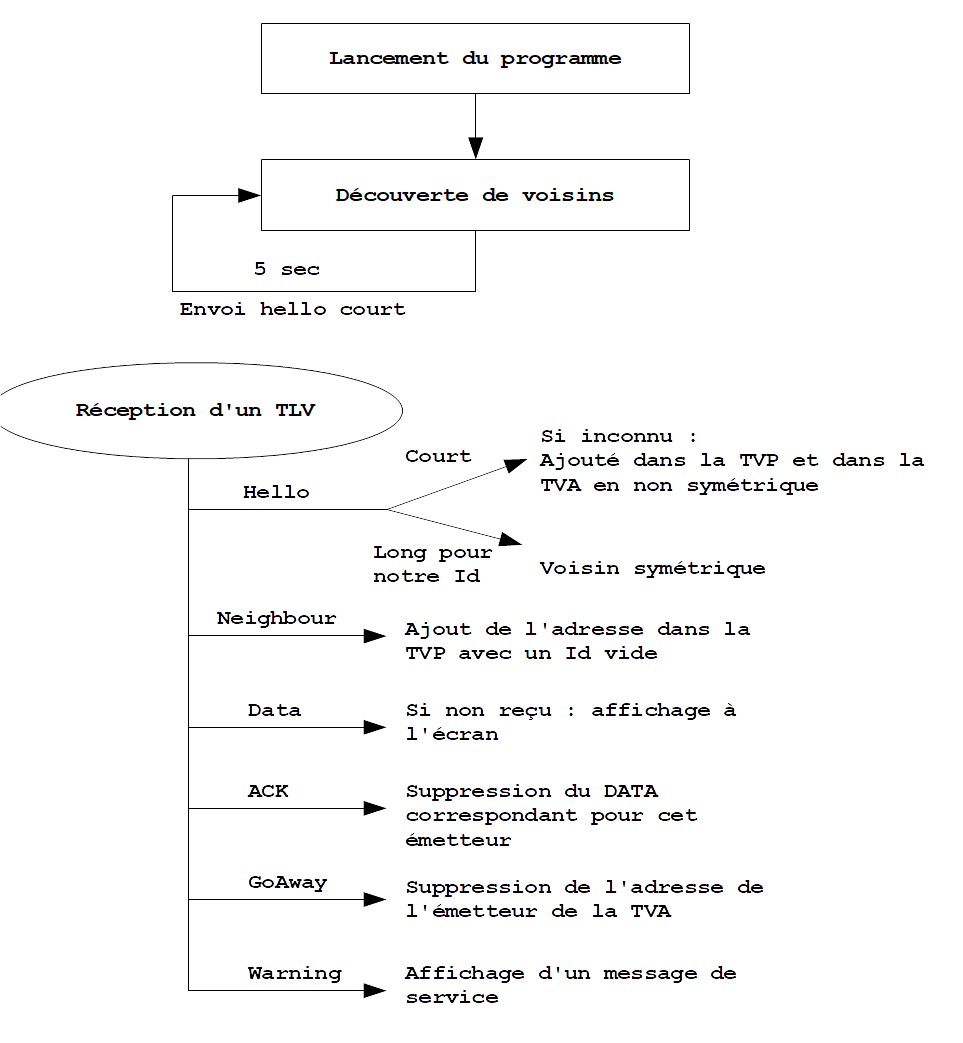
\includegraphics[width=.8\columnwidth]{img.png}
		\label{fig:img}
		\caption{Vue d'ensemble résumée de l'algorithme}
	\end{figure}
	
	Quelques détails de gestion, notamment concernant les délais d'envoi:
	
	\begin{itemize}
		\item 	Les TLV en attente (Data et Neighbour) sont envoyés toutes les 5 secondes, et les Hello courts toutes les 5 secondes également (en multicast, de façon 	directe sans passer par la mise en attente).
	
	\item On supprime le voisin de la TVA lors de la réception d'un GoAway de sa part.
	
	\item Toutes les 20 secondes, nettoyage de la table des données récemment reçues (la durée de vie de chaque donnée est de 3 minutes).
	
	\item Sur réception d'un Hello court, envoi d'un Hello long à cette personne s'il n'est pas dans notre table d'actifs.
	
	\item  Toutes les secondes, la table TVA est parcourue et les statuts de symétrie sont mis à jour selon l'instant de réception du dernier hello long.
	Des voisins sont supprimés s'ils sont inactifs.

	\end{itemize}
	
	\subsection{Erreurs}
	
	Le programme a été testé sur les systèmes de la salle informatique de l'ENS (des Linux basés sur Debian type Ubuntu), à distance avec \emph{Secure Shell}.
	Le multicast a donc été testé dans la limite de la salle (un commutateur assurant la liaison).
	
	Pendant ces séances de test, quelques fois, un voisin potentiel fantôme s'immisce dans la TVP (il ne correspond pas aux adresses IP connues). Ce voisin n'envoie
	jamais de Hello...
	
\section{Conclusion}
	
	Le développement d'un tel utilitaire a permis de mettre en œuvre la plupart des notions vues au cours du semestre dans le cours
	de réseau : transfert de données avec UDP, l'utilisation d'IPv6 et le \emph{multicast} amélioré que cette norme permet, mais aussi les rudiments
	 de programmation système et de gestion bas niveau de la machine.
	
	Une des perspectives serait de sécuriser totalement le programme (quelques cas d'erreurs de dépassement subsistent envers et contre tout), pour ensuite
	ouvrir la voie à des applications de plus haut niveau : le transfert de fichier comme vu plus haut, ou la messagerie pair à pair privée par exemple.
	
	\medskip
	
	Enfin d'un point de vue plus pratique, le code pourrait être clarifié et mieux organisé. En effet et malgré nos efforts, certaines parties sont peu commentées
	ou documentées. Néanmoins nous avons documenté les fonctions les plus importantes (à l'aide du style XML/MSDN/Doxygen), et nous nous sommes appliqués à
	utiliser une convention de nommage cohérente.
\end{document}